% This must be in the first 5 lines to tell arXiv to use pdfLaTeX, which is strongly recommended.
\pdfoutput=1
% In particular, the hyperref package requires pdfLaTeX in order to break URLs across lines.

\documentclass[11pt]{article}

% Remove the "review" option to generate the final version.
\usepackage[review]{EMNLP2023}

% Standard package includes
\usepackage{times}
\usepackage{latexsym}

% For proper rendering and hyphenation of words containing Latin characters (including in bib files)
\usepackage[T1]{fontenc}
% For Vietnamese characters
% \usepackage[T5]{fontenc}
% See https://www.latex-project.org/help/documentation/encguide.pdf for other character sets

% This assumes your files are encoded as UTF8
\usepackage[utf8]{inputenc}

% This is not strictly necessary and may be commented out.
% However, it will improve the layout of the manuscript,
% and will typically save some space.
\usepackage{microtype}

% This is also not strictly necessary and may be commented out.
% However, it will improve the aesthetics of text in
% the typewriter font.
% \usepackage{inconsolata}

\usepackage{microtype}
\usepackage{enumitem}
\usepackage{times}
\usepackage{latexsym}
\usepackage{xspace}
\usepackage{booktabs}
\usepackage{multirow}
\usepackage{makecell}
\usepackage{color}
\usepackage{microtype}
\usepackage{amsmath}
\usepackage{graphicx}
\usepackage{amssymb,amsthm}
\usepackage{xcolor}
\usepackage{subcaption}
\usepackage{caption}
%\usepackage{paralist}
\usepackage{cleveref}
\usepackage{booktabs}
\usepackage{url}
\usepackage[normalem]{ulem}
\useunder{\uline}{\ul}{}
\newcommand{\todo}[1]{{\color{red}{#1}}}
\newcommand{\our}{\mbox{\textsc{DocSplit}}}
\newcommand{\ourbert}{$\our_{\mathrm{bert}}$}
\newcommand{\ourlong}{$\our_{\mathrm{long}}$}
% If the title and author information does not fit in the area allocated, uncomment the following
%
%\setlength\titlebox{<dim>}
%
% and set <dim> to something 5cm or larger.

\title{DocSplit: Simple Contrastive Pretraining for \\ Large Document Embeddings}

% Author information can be set in various styles:
% For several authors from the same institution:
% \author{Author 1 \and ... \and Author n \\
%         Address line \\ ... \\ Address line}
% if the names do not fit well on one line use
%         Author 1 \\ {\bf Author 2} \\ ... \\ {\bf Author n} \\
% For authors from different institutions:
% \author{Author 1 \\ Address line \\  ... \\ Address line
%         \And  ... \And
%         Author n \\ Address line \\ ... \\ Address line}
% To start a separate ``row'' of authors use \AND, as in
% \author{Author 1 \\ Address line \\  ... \\ Address line
%         \AND
%         Author 2 \\ Address line \\ ... \\ Address line \And
%         Author 3 \\ Address line \\ ... \\ Address line}

% \author{First Author \\
%   Affiliation / Address line 1 \\
%   Affiliation / Address line 2 \\
%   Affiliation / Address line 3 \\
%   \texttt{email@domain} \\\And
%   Second Author \\
%   Affiliation / Address line 1 \\
%   Affiliation / Address line 2 \\
%   Affiliation / Address line 3 \\
%   \texttt{email@domain} \\}

\author{Yujie Wang \\
  Claremont Graduate University 
  \texttt{yujie.wang@cgu.edu} \\\And
  Mike Izbicki \\
  Claremont McKenna College
  \texttt{Michael.Izbicki@ClaremontMcKenna.edu} \\}

\begin{document}
\maketitle
\begin{abstract}

Existing model pretraining methods only consider local information.
For example, in the popular token masking strategy, the words closer to the masked token are more important for prediction than words far away.
This results in pretrained models that generate high-quality sentence embeddings, but low-quality embeddings for large documents.
We propose a new pretraining method called $\our$ which forces models to consider the entire global context of a large document.
Our method uses a contrastive loss where the positive examples are randomly sampled sections of the input document, and negative examples are randomly sampled sections of unrelated documents.
Like previous pretraining methods, $\our$ is fully unsupervised, easy to implement, and can be used to pretrain any model
architecture.
Our experiments show that $\our$ outperforms other pretraining methods for document classification, few shot learning, and information retrieval tasks.
\end{abstract}



\section{Introduction}

Generating high-quality text embeddings for documents is a long-standing open problem.
Most previous studies focus on either learning sentence-level representations~\cite{Hill2016LearningDR, Logeswaran2018AnEF, Gao2021SimCSESC} where training data usually contain short text or designing specific model structures for larger-range dependencies~\cite{Beltagy2020LongformerTL, Zaheer2020BigBT},
but effective and efficient document representation learning methods are less explored.

\begin{figure}[h]
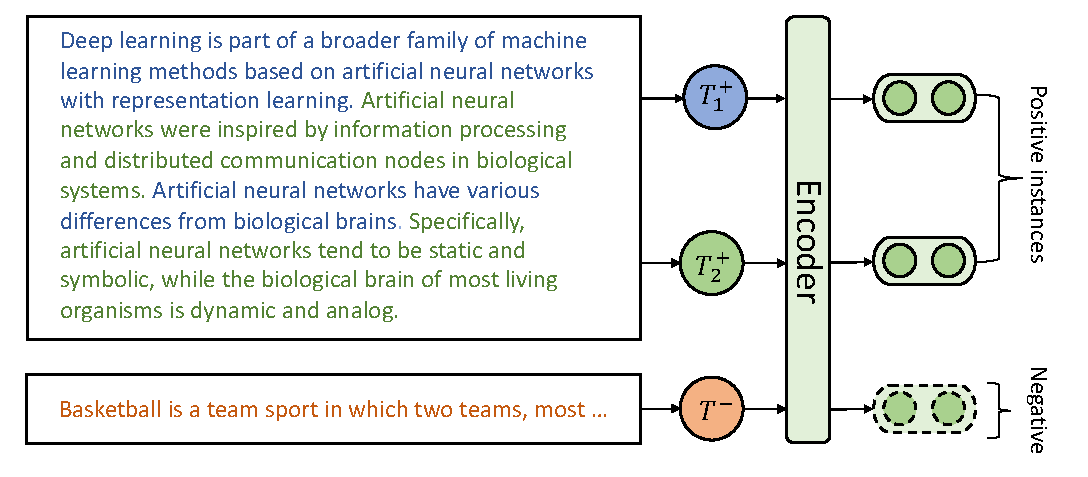
\includegraphics[width=\columnwidth]{fig/docsplit.pdf}
\caption{Overall framework of \our. The document is randomly divided into two exclusive subsets of sentences and the two subsets work as positive pairs for contrastive learning. Other instances in the same batch are used as negatives.
}
\label{overall}
\end{figure}

In this paper, we present the $\our$ which is the first unsupervised pretraining method designed specifically for large documents.
The training procedure of $\our$ can work with any model architecture to improve document representations. 
Specifically, $\our$ uses contrastive learning,
and our key contribution is a new method for generating positive samples for contrastive learning.
To this end, we first investigate the information redundancy with two methods (details in Appendix~\ref{app:redundacy}) on five datasets for different lengths of documents.
We find (1) information redundancy is larger as the length of the documents is increasing and (2) sentences from the same document usually contain repeated information. 
Based on this observation, we can assume that the model can still learn the semantics of documents even if we drop some sentences. Hence, as shown in Figure~\ref{overall}, we randomly divide the original documents into two parts by sentences as positive pairs. Due to redundancies, our model can still recognize the two pairs have the same semantics. 
The intuition behind this method is that we expect the model will pull representations of two subsets together in the latent space by paying more attention to common keywords so that the model can learn key information from documents automatically. 

To evaluate the quality of document embeddings, we conduct standard and few-shot text classification on five large document datasets involved in News and scientific articles. Moreover, to further validate the effectiveness of our method, we also conduct document retrieval on the AAN dataset which is designed for long document understanding evaluation.
The experimental results show that \our~with two kinds of model structures (i.e.,~BERT and Longformer) can both achieve significant improvements compared to state-of-the-art baselines.

% The recurrent connections in models like the LSTM~\cite{Hochreiter1997LongSM} and GRU~\cite{Cho2014OnTP} allow information at all locations in the document to influence the final embedding,
% but they are slow to train because the models must consider each word sequentially.
% The Transformer architecture~\cite{Vaswani2017AttentionIA} uses self-attention with no recurrent connections,
% and so can be trained much faster than recurrent models.
% This has led to the widespread use of language models like BERT~\cite{Devlin2019BERTPO} and ELMO~\cite{Peters2018DeepCW} that are pre-trained on large scale web data.
% Unfortunately, the memory requirements of self-attention scale as $O(n^2)$ and so are not suitable for long documents.
%Large scale pre-trained transformers like BERT~\cite{} and ELMO~\cite{} are currently state-of-the-art for many NLP tasks that require only short-term dependencies in text.
%These transformers do not handle long-term dependencies well, however, because they require $O(n^2)$ memory for the size of the context window.
% The LongFormer~\cite{Beltagy2020LongformerTL} and BigBird~\cite{Zaheer2020BigBT} models allow larger-range dependencies by introducing improved attention mechanisms that reduce the memory requirements down to $O(n)$.
% This previous research focuses on designing new model architectures suitable for long text,
% but in this paper we present the $\our$ training procedure that can work with any model architecture.
%All of this previous research focuses on designing new model architectures.
%Our paper introduces a new training method called the $\our$ that works for any model architecture.



% $\our$ is the first unsupervised training method designed specifically for long text.
% Previous methods for training on long text either require supervision~\cite{} or use the masked language modeling (MLM) technique~\cite{}.
% In MLM, we replace a token from the input text with a special ``mask'' token and train the model to predict which token was removed.
% The MLM pretraining method has been shown to work well for short-text documents~\cite{},
% but we argue that it sub-optimal for long text because most of the information for predicting the masked token is available near the token.
% The $\our$ pretraining technique is designed to force the model to learn long range dependencies within a document.
% Specifically, $\our$ uses contranstive learning,
% and our key contribution is a new method for generating the positive samples for contrastive learning (see Figure~\ref{overall} above).
%The most similar work to our own is the \texttt{SimCSE} method which uses contrastive learning to pre-train text models,

%Supervised methods cannot be used for large-scale pretraining of models, however, so we present the 

Our paper is organized as follows.
In Section~\ref{sec:method} we formally define the contrastive learning problem and our novel $\our$ training method.
%We highlight how our $\our$ method improves on related contrastive learning frameworks like \texttt{SimCSE}
In Section~\ref{sec:experiments} we develop a new experimental evaluation procedure for documents.
We conclude in Section~\ref{sec:conclusion} by emphasizing that all of our models and datasets are open source.

\section{Method}

\label{sec:method}
In this section, we first formally define contrastive learning, then we describe our \our~method.
\subsection{Contrastive Learning}
Contrastive Learning aims to learn effective representations by pulling semantically close neighbors together and pushing apart non-neighbors in the latent space~\cite{Hadsell2006DimensionalityRB}.
It assumes a contrastive instance $\{x, x^{+}, x_1^{-},\dots,x_{N-1}^{-}\}$ including one positive and $N-1$ negative instances and their representations $\{\mathbf{h}, \mathbf{h}^{+}, \mathbf{h}_1^{-}, \dots,
\mathbf{h}_{N-1}^{-}\}$, where $x$ and $x^{+}$ are semantically related.
we follow the contrastive learning framework~~\cite{Chen2020ASF, Li2022UCTopicUC} and take cross-entropy as our objective function:
\begin{equation}
\label{cl}
    l = -\log \frac{e^{\mathrm{sim}(\mathbf{h}, \mathbf{h}^{+})/\tau}}{e^{\mathrm{sim}(\mathbf{h}, \mathbf{h}^{+})/\tau}+ \sum_{i=1}^{N-1}e^{\mathrm{sim}(\mathbf{h}, \mathbf{h}_i^{-})/\tau}}
\end{equation}
where $\tau$ is a temperature hyperparameter and $\mathrm{sim}(\mathbf{h}_1, \mathbf{h}_2)$ is the cosine similarity $\frac{\mathbf{h}_1^{\top}\mathbf{h}_2}{\Vert \mathbf{h}_1 \Vert \cdot \Vert \mathbf{h}_2 \Vert}$.
In this work, we encode input texts using a pre-trained language model such as BERT~\cite{Devlin2019BERTPO}. Following BERT, we use the first special token \texttt{[CLS]} as the representation of the input and fine-tune all the parameters using the contrastive learning objective in Equation~\ref{cl}.

\subsection{DocSplit}
The critical problem in contrastive learning is how to construct positive pairs $(x, x^{+})$.
In representation learning for visual tasks~\cite{Chen2020ASF}, an effective solution is to take two random transformations of the same image (e.g.,~flipping, rotation).
Similarly, in language representations, previous works~\cite{Gao2021SimCSESC, Karpukhin2020DensePR, Meng2021COCOLMCA, Li2022UCTopicUC} apply augmentation techniques such as dropout, word deletion, reordering, and masking.

In this paper, we propose a new method to construct positive instances for documents. 
The basic idea of positive instance construction for contrastive learning is adding random noises to the original data for augmentation. 
The augmented data should have similar representations to the original data. 
Models trained by contrastive losses on augmented data will have an increased ability to learn important features in the data.
To add random noises in documents, we find documents usually has higher information redundancy than sentences (Table~\ref{redundancy} in Appendix). 
With this observation, we can have an assumption: 
the semantics of a document will not be changed even if we drop half of the document. 
We can construct positive pairs under this assumption easily on any text dataset without supervision.
Specifically, for each document in the dataset, we randomly split sentences in the document into two subsets and the two sentence sets do not have intersections. 
In the two subsets, we keep the order of sentences in the original document to form two new documents. 
According to our assumption, the two new documents should have the same semantics and hence they are used as a positive pair in contrastive learning. 

Consider an example (in Figure~\ref{overall}) to understand our positive instance construction process:
Suppose we have a document $T = (s_1, s_2,\dots,s_n)$ where $s_i$ is the $i$-th sentence in document and $n$ is the number of sentences, each sentence will be sent to anchor set or positive set with the same probability ($50\%$). 
The sentences in the same set (i.e.,~anchor or positive) will be concatenated in the same order of $T$ to form one positive pair $(T^+_1, T^+_2)$ for contrastive learning. 
Positive pairs constructed by this method will not contain the same sentence and hence prevent models from overfitting on recognizing the same sentences. 
Instead, models are guided to learn keywords appearing in positive instances so as to improve the ability to recognize key information. 
We split the document at sentence level instead of word level (e.g.,~word deletion for augmentation) because the word-level splitting will cause the discrepancy between pretraining and finetuning and then lead to performance decay.

For negative instances, we use in-batch instances following previous contrastive frameworks~\cite{Gao2021SimCSESC, Li2022UCTopicUC}.



\section{Experiments}

\label{sec:experiments}

We perform a careful ablation study to isolate the effects of the $\our$ pretraining method on downstream task performance.
First, we generate two different sets of baseline models: one for models using the contrastive loss, and one for models designed for large document embeddings.
We pretrain separate models for each group of baselines.
Then, we perform downstream experiments on standard classification, few-shot learning, and information retrieval tasks.
In all cases, models pretrained with $\our$ outperform models pretrained with other methods.

%We first describe how we pretrain our model.
%Then we describe our classification, few-shot learning, and information retrieval evaluation tasks.

%We use a standard experimental setup to evaluate the effectiveness of \our.
%First, we pretr
%
%We evaluate the effectiveness of \our~using a standard procedureby pretraining two models on English language wikipedia.
%Then we finetune the model
%
%In this section, we evaluate the effectiveness of our method by conducting text classification tasks. 
%To eliminate the influence of different model structures and focus on the quality of text embeddings. 
%We freeze the parameters of different text encoders and fine-tune only a multi-layer perceptron (MLP) to classify the embeddings of text encoders.
%We also visualize the attention weights between baselines and \our.
%
%We do not use semantic textual similarity (STS) tasks~\cite{Agirre2012SemEval2012T6} because the sentences in these tasks are short which is not suitable to evaluate large document embeddings.
\begin{table*}
    \centering
% \scalebox{0.7}{
% \setlength{\tabcolsep}{1.mm}{
    %\begin{tabular}{@{}lR{0.75in}R{0.75in}R{0.75in}R{0.75in}R{0.75in}R{0.75in}@{}}
\small
\begin{tabular}{l|cccccccccc}
\toprule
 Datasets   & \multicolumn{2}{c}{FakeNews}     & \multicolumn{2}{c}{20News}         &\multicolumn{2}{c}{arXiv}     &\multicolumn{2}{c}{NYT}        & \multicolumn{2}{c}{BBCNews} \\
 \cmidrule(l){1-1} 
\cmidrule(l){2-3} 
\cmidrule(l){4-5}
\cmidrule(l){6-7}
\cmidrule(l){8-9}
\cmidrule(l){10-11}
Metrics    & Acc & F1   & Acc & F1    & Acc & F1    & Acc & F1      & Acc & F1 \\

\midrule
\multicolumn{11}{c}{\textit{Text Classification}}   \\
\midrule
BERT      &54.98  &42.17    &62.34  &54.19    &68.52  &20.46     &95.11  &92.65      &91.06  &90.34 \\
CT-BERT       &55.19  &42.53    &65.76  &63.37  &71.61 &26.09  &95.69  &91.59  &90.32  &88.87   \\
SimCSE &58.48  &47.46    &74.02  &72.57    &74.46  &30.01     &97.17  &94.69      &94.12  &93.86  \\
SimCSE$_{\mathrm{long}}$ &58.37  &47.56    &73.51  &72.05    &73.16 &29.41  &97.25 &93.83   &94.22  &94.30 \\
cpt-text  & &  & &  \\
INSTRUCTOR  & &  &\textbf{80.62} &\textbf{78.72} &75.52 &30.46 &97.06 &93.66 &95.19 &95.16 \\
\our$_{\mathrm{bert}}$        &\textbf{60.04}  & \textbf{50.14}   &76.89  &74.85   &\textbf{76.66}  &\textbf{32.24}     &\textbf{98.20}  &\textbf{96.05}      &\textbf{95.56}  &\textbf{95.58}  \\
\midrule
LongFormer  &65.72  &57.66    &73.69  &72.47    &71.66  &25.92     &94.36  &88.39      &96.33  &94.75  \\
BigBird      &57.44  &47.87    &70.35  &68.91    &71.58 &25.05  &97.13 &94.33   &94.11  &94.62 \\
\our$_{\mathrm{long}}$  &\textbf{71.60}   &\textbf{61.66}     &\textbf{75.44}  &\textbf{74.38}    &\textbf{77.68}  &\textbf{33.26}     &\textbf{97.90}  &\textbf{95.43}  &\textbf{96.67}  &\textbf{95.91}  \\


\midrule
\multicolumn{11}{c}{\textit{Few-shot Text Classification}}   \\
\midrule
BERT      &23.96  &23.73    &19.94  &18.71    &24.08  &10.14     &51.85  &43.90      &54.22  &52.73 \\
CT-BERT      &23.71  &23.06    &24.11  &23.53    &27.02  &13.53     &47.23  &36.83      &59.56  &58.95   \\
SimCSE      &25.04  &22.68    &42.63  &41.42    &32.61  &17.19     &86.51  &78.41      &83.56  &83.75    \\
SimCSE$_{\mathrm{long}}$ &26.39  &23.26    &48.65  &47.81    &23.42 &12.66  &85.36 &75.90   &84.44  &83.96 \\
\our$_{\mathrm{bert}}$  &\textbf{27.79}  &\textbf{24.65}    &\textbf{55.79}  &\textbf{55.43}    &\textbf{35.79}  & \textbf{18.52}    &\textbf{90.52}  &\textbf{83.71}      &\textbf{86.86}  &\textbf{86.31}   \\
\midrule
LongFormer  &26.56  &25.12    &44.42  &42.41    &25.04  &13.36     &73.06  &54.87      &84.89  &85.47  \\
BigBird      &25.36  &23.28    &39.14  &39.06    &23.62 &10.18  &86.66 &78.96   &79.11  &76.63 \\
\our$_{\mathrm{long}}$  &\textbf{29.17}  &\textbf{27.13}    &\textbf{51.18}  &\textbf{50.96}    &\textbf{34.33}  &\textbf{18.80}   &\textbf{89.78}  &\textbf{82.88}      &\textbf{86.78}  &\textbf{86.66}  \\
\bottomrule
\end{tabular}
    % }}
    \caption{Larger numbers are better. Our pre-trained model achieves the best results in all cases.}
    \vspace{-3mm}
    \label{results}
\end{table*}

\subsection{Baselines}

%In order to demonstrate that $\our$ is widely applicable,
%we pretrain two models using two different architectures.

All existing models pretrained with a contrastive loss are pretrained on the standard bert \cite{Devlin2019BERTPO} architecture.
We therefore also pretrain a model using the bert architecture,
and we call the resulting model \ourbert.
The models trained with a contrastive loss that we compare \ourbert~to are SimCSE \cite{Gao2021SimCSESC}, CT-BERT~\cite{Carlsson2021SemanticRW}, Contriever~\cite{Izacard2021UnsupervisedDI} and INSTRUCTOR~\cite{Su2022OneEA}.\footnote{We do not compare to the popular RoBERTa~\cite{Liu2019RoBERTaAR}, IS-BERT~\cite{Zhang2020AnUS} and GTR~\cite{Ni2021LargeDE} models because SimCSE and INSTRUCTOR achieve better results than these methods according to their papers.}
We will see that on all of our large document tasks, \ourbert~outperforms each of these other models.
%Therefore, any performance differences we observe in model performance must be due to the pretraining method.

We call the second model \ourlong~because it is pretrained on the LongFormer architecture \cite{Beltagy2020LongformerTL}.
LongFormer uses a modified attention head that requires only $O(n)$ compute instead of the standard $O(n^2)$ that Bert uses,
and so can handle larger context windows needed for large documents.
Our \ourlong pretrained model inherits this computational advantage.
We also compare to the BigBird~\cite{Zaheer2020BigBT} model,
which is architecturally similar.

\subsection{Pretraining Details}

To pretrain both models, we follow the standard pretraining procedure for contrastive losses established by \citet{Gao2021SimCSESC} and \citet{Li2022UCTopicUC}.
We simultaneously optimize both the masked language model (MLM) loss (with weight$=0.1$) and the contrastive loss (with temperature $\tau=0.05$).
We use English Wikipedia articles as our pretraining dataset.
These articles are long, and so we expect that a pretraining procedure designed for large documents will improve performance.
The total number of training instances is 6,218,825.
We use AdamW \cite{Kingma2014AdamAM} with a learning rate of 5e-5.
\ourbert uses a batch size of 36.
And due to the larger memory requirements of the LongFormer architecture,
\ourlong uses a batchsize of 12.
For both models, we know that performance improvements on downstream tasks must be due to the pretraining procedure and not the dataset because all baseline models include English language wikipedia in their training set.

%\subsection{Baselines}
%
%We compare our two pre-trained model to baselines with similar architectures and different pretraining strategies.
%
%
%For \ourbert
%(1) Language models trained for general language understanding and sentence embeddings include BERT~\cite{Devlin2019BERTPO}, SimCSE~\cite{Gao2021SimCSESC}~\footnote{SimCSE can be viewed as an ablation model without document splitting.}, CT-BERT~\cite{Carlsson2021SemanticRW}, Contriever~\cite{Izacard2021UnsupervisedDI} and INSTRUCTOR~\cite{Su2022OneEA}. 
%For a fair comparison, we also train a SimCSE with our pretraining dataset (SimCSE$_\mathrm{long}$).
%(2) Transformers specified for long sequences include Longformer~\cite{Beltagy2020LongformerTL} and BigBird~\cite{Zaheer2020BigBT}.
%We train two versions of \our~with BERT and Longformer (i.e.,~\our$_\mathrm{bert}$ and \our$_{\mathrm{long}}$) for comparison.


\subsection{Text Classification}
In the standard text classification task, we classify text embeddings with the full training set. 
Training details are in Appendix~\ref{app:details}.

\textbf{Datasets.}
We use the following classic documents datasets to evaluate our method:
(1) Fake News Corpus~\footnote{https://github.com/several27/FakeNewsCorpus};
(2) 20NewsGroups~\cite{Lang1995NewsWeederLT};
(3) arXiv articles dataset~\footnote{https://www.kaggle.com/datasets/Cornell-University/arxiv};
(4) New York Times Annotated Corpus (NYT) ~\cite{sandhaus2008new}; and
(5) BBCNews~\footnote{http://mlg.ucd.ie/datasets/bbc.html}.

%\begin{table}[t]
%\centering
{
\small
\begin{tabular}{lrrrrrrrr}
\toprule
Dataset & Num Docs & Classes & \multicolumn{2}{c}{Words~/~Doc} &99th &95th &90th &75th \\
    \cmidrule{4-5}
& & & Mean&  Max \\
\midrule
FakeNews &8,558,957 &15 &467 &33,936 &2,949 &1,403 &1,024 &608 \\
arXiv &2,162,833 &38 &138 &925 &289 &255 &230 &181 \\
20News &18,846 &20 &258 &11,554 &1,865 &714 &468 &264\\
NYT &13,081 &5 &650 &5503 &1,264 &1,043 &966 &831\\
BBCNews &2,225 &5 &133 &445 &311 &234 &206 &167\\
\bottomrule
\end{tabular}
}

%\label{dataset}
%\end{table}

\textbf{Results.}
Table~\ref{results} shows the evaluation results on different datasets. 
Overall, we can see that \our~achieves the best performance over the 4 document datasets (except INSTRUCTOR on 20News due to its data leakage) and consistently improves the document embeddings with BERT and Longformer structures. 
INSTRUCTOR~\cite{Su2022OneEA} includes 20News in their pretraining datasets which causes data leakage in our experiments, hence INSTRUCTOR results on 20News are not comparable to others.
Specifically, methods pretrained with contrastive objectives (i.e.,~CT-BERT, SimCSE, Contriever and INSTRUCTOR) outperform general language representations (i.e., BERT and LongFormer) which indicates contrastive objectives designed for text embeddings can largely improve the ability of language models to produce high-quality text embeddings. 
SimCSE pretrained with our document data (i.e.,~SimCSE$_{\mathrm{long}}$) has similar results as the original SimCSE which indicates simply increasing the length of pretraining text cannot improve document embeddings.
Under the same model structures, our model achieves $3.9\%$ and $9.4\%$ average macro-F1 improvements with BERT and Longformer structures respectively compared to SimCSE and Longformer. 
Compared to the state-of-the-art model INSTRUCTOR, our model (\our$_{\mathrm{bert}}$) can achieve $3.4\%$ improvements.
Hence, our contrastive learning method is effective for document embeddings.


\subsection{Few-shot Text Classification}
To show the performance of different text embeddings under low-resource settings, we evaluate our model with few-shot training instances.
Training details are in Appendix~\ref{app:details}.

\begin{figure}
\centering
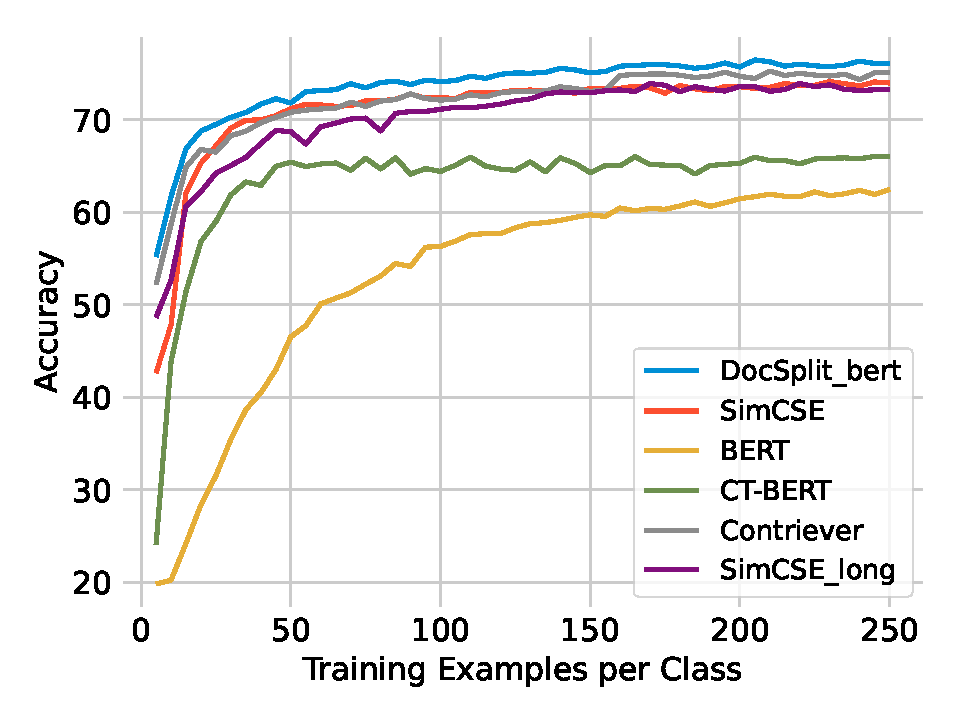
\includegraphics[width=0.8\linewidth]{fig/few_shot.pdf}
\caption{Performance of different models with different numbers of instances per class under few-shot setting.}
\label{few_shot}
\end{figure}

\textbf{Results.} 
Table~\ref{results} shows the results of few-shot text classification on these five datasets. 
We can see that, under the same model structure, \our~(i.e.,~\our$_{\mathrm{bert}}$ and \our$_{\mathrm{long}}$) achieves $12.0\%$ and $24.3\%$ macro-F1 improvements compared to SimCSE and Longformer respectively. 
Surprisingly, INSTRUCTOR achieves low performance on the NYT and BBCNews under few-shot settings.
%and achieves 0.028+0.082+2.03+0.769. 
These improvements are higher than standard text classification. 
Besides, we also compare the performance of different baselines (using BERT as a backbone) and \our$_{\mathrm{bert}}$ with different numbers of training instances on 20News. 
The results in Figure~\ref{few_shot} show the improvements from our method become larger as the number of training instances decreases indicating the importance of high-quality document embeddings for low-resource settings. 
Furthermore, our method achieves the best results under different numbers of training instances.

\subsection{Document Retrieval}
We conduct document retrieval to evaluate the ability to learn the similarity score between two vectors~\cite{Guo2016ADR} of documents. We follow the document retrieval experiment~\cite{Tay2020LongRA} and use the ACL Anthology Network (AAN)~\cite{Radev2009TheAA} dataset, which identifies if two papers have a citation link, a common setup used in long-form document matching~\cite{Jiang2019SemanticTM,Yang2020Beyond5T}.
Specifically, for all baselines, we use models to obtain document embeddings and finetune an MLP layer on two concatenated embeddings to predict if two documents have a citation link.

\textbf{Results.} 
\begin{table*}
    \centering
    \small
\begin{tabular}{l|c}
\toprule
Model   & Retrieval\\

\midrule
BERT   &53.56  \\
CT-BERT     &54.23 \\
SimCSE   &54.78\\
SimCSE$_{\mathrm{long}}$ &55.23 \\
cpt-text                   \\
INSTRUCTOR                 \\
\our$_{\mathrm{bert}}$   &58.29  \\
\midrule
LongFormer  &56.89  \\
BigBird     &59.29 \\
\our$_{\mathrm{long}}$  &59.89  \\
\bottomrule
\end{tabular}
    \caption{}
    \vspace{-3mm}
    \label{retrieval}
\end{table*}
Table~\ref{retrieval} shows the results of the document retrieval experiment on AAN dataset.
We can find that our method achieves the best results due to the effectiveness of our pretraining methods based on document splitting.

\section{Conclusion}
\label{sec:conclusion}
In this work, we propose an unsupervised contrastive learning framework for large document embeddings. 
Our paper provides a new method for large document data augmentation without any supervision and language models can get large-scale pretraining on any large documents. 
We conduct extensive experiments on text classification tasks under fully supervised and few-shot settings and a document retrieval task for further evaluation.
Results show that our pre-trained model greatly outperforms state-of-the-art text embeddings, especially when the training data is limited.

\section*{Limitations}
The limitations of our method are as follows:
\begin{enumerate}[nosep,leftmargin=*]
    %\item Our method requires human-annotated data, which is expensive and time-consuming.
    \item Generative models cannot be trained using $\our$, but they can be trained using token masking.
    \item We do not know how $\our$ will generalize to extremely large documents (e.g.\ book length).
        We lack the computational resources to train models on these larger documents.
\end{enumerate}

\section*{Ethics Statement}
We do not anticipate any major ethical concerns; learning document embedding is a fundamental problem in natural language processing. Ethical considerations seem low-risk for the specific datasets studied here because they are all published.

%\section*{Acknowledgements}

% Entries for the entire Anthology, followed by custom entries
\bibliography{anthology,custom}
\bibliographystyle{acl_natbib}

\clearpage
\appendix
\section{Appendix}

\subsection{Related Work}

\textbf{Text Embeddings}. Learning text embeddings is a fundamental task in natural language processing (NLP) which can be used in information retrieval~\cite{Thakur2021BEIRAH}, text similarity~\cite{Gao2021SimCSESC}, classification~\cite{Minaee2021DeepLB}, etc. Existing works focus on learning general text embeddings for different applications. SimCSE~\cite{Gao2021SimCSESC} augment training data by Dropout~\cite{Srivastava2014DropoutAS} to construct positive data for contrastive learning. Sentence-BERT~\cite{Reimers2019SentenceBERTSE} employs siamese and triplet network structures to compare the labeled sentences in the natural language inference (NLI) dataset. Contriever~\cite{Izacard2021UnsupervisedDI} learns text embeddings for information retrieval via contrastive learning considering multilingual corpus. INSTRUCTOR~\cite{Su2022OneEA} collects a massive dataset from 330 diverse NLP tasks and formulates all tasks into information retrieval tasks with prompts. 
Previous works either rely on massive manually annotated data~\cite{Su2022OneEA, Reimers2019SentenceBERTSE} or focus only on short text (i.e.,~sentences) embeddings~\cite{Gao2021SimCSESC}.
In this paper, we study unsupervised representation learning of document embeddings which usually have longer text than general sentence embeddings and this task brings new challenges for models to understand a document.

\textbf{Model Structures for Documents}. Due to the limitations of Transformer~\cite{Vaswani2017AttentionIA} on long documents, Another line of work studies the efficient model structures which can be effective to encode documents. For example, Longformer~\cite{Beltagy2020LongformerTL} introduces an attention mechanism that scales linearly with sequence length, making it easy to process long documents. BigBird~\cite{Zaheer2020BigBT} proposes a sparse attention mechanism that reduces this quadratic dependency to linear. \citet{Bulatov2022RecurrentMT} combines the memory mechanism in LSTM~\cite{Hochreiter1997LongSM} with Transformer to let transformers encode extremely long sequences. Comparing these methods which focus on designing models for long documents, our work studies the effective training method for long documents which can be adopted to any model structures for pre-training.


\subsection{Redundancy}
\label{app:redundacy}
\begin{table}[t]
    \small
\begin{tabular}{l|cccccc}
\toprule
Length   & (1) & (2) & (3)   &  (4) &  (5)  & All\\
\midrule
FakeNews &1.06 &1.21 &29 &1.35 &1.52 &1.37 \\
20News &1.12 &1.18 &1.24 &1.31 &1.50 &1.28 \\
arXiv &1.12 &1.25 &1.36 &1.49 &1.62 &1.34\\
NYT &1.00 &1.14 &1.21 &1.31 &1.48 &1.45\\
BBCNews &1.05 &1.14 &1.20 &1.29 &1.46 &1.19 \\
\bottomrule
\end{tabular}
    \caption{Information redundancies for different lengths (i.e.,~word numbers) of text: (1) 0-50 (2) 51-100 (3) 101-200 (4) 201-300 (5) more than 300.}
    \label{redundancy}
\end{table}

We evaluate the redundancy of the text by two methods: (1) counting the repeated verbs and nouns in the text; (2) comparing inner-document and inter-document sentence similarities.

For (1), we first use SpaCy~\footnote{https://spacy.io/} to find verbs and nouns and get their lemmatizations. Intuitively, if the redundancy of a document is high, nouns and verbs will be repeated frequently to express the same topic. Hence, redundancies $R$ in our paper are computed as:
\begin{equation}
    R = \frac{N_{\mathrm{nouns, verbs}}}{D_{\mathrm{nouns, verbs}}}
\end{equation}
where $N_{\mathrm{nouns, verbs}}$ denotes the number of nouns and verbs in a document and $D_{\mathrm{nouns, verbs}}$ is the number of distinct nouns and verbs.

For (2), we compute sentence similarities to compare inner-document and inter-document information. Specifically, we first split documents into sentences and encode these sentences with pre-trained SimCSE~\cite{Gao2021SimCSESC}. Then, we calculate cosine similarities for every two sentences in the same documents (i.e.,~inner-document) and from different documents (i.e.,~inter-document). Results from five datasets are shown in Table~\ref{sent_sim}. We can see that sentences in the same documents have higher similarities compared to sentences from different documents. These results show that sentences in the same documents usually contain repeated information and hence have higher redundancy (i.e.,~sentences expressing similar semantics).

\label{app:sent_sim}
\begin{table}[t]
    \small
\begin{tabular}{l|cccccc}
\toprule
Sentence Similarity  &Inner-Document  &Inter-Document\\
\midrule
FakeNews &0.28 &0.06 \\
20News &0.21 &0.07 \\
arXiv &0.51 &0.35\\
NYT &0.30 &0.11 \\
BBCNews &0.32 &0.09 \\
\bottomrule
\end{tabular}
    \caption{Inner-document and inter-document sentences similarities measured by SimCSE.}
    \label{sent_sim}
\end{table}

\subsection{Training Details}
\label{app:details}
For text classification, the learning rate for fine-tuning is 3e-4; the batch size is 8; the maximum sequence length is 512 tokens. 
We fine-tune the last MLP layer on these five datasets and evaluate the classification performance with accuracy and macro-F1 scores.
For few-shot text classification, we sample 10 data instances per class for the FakeNewsCorpus dataset and the arXiv dataset and 5 data instances per class for the other three datasets. 
Other settings are the same as the standard text classification. 
Since there is randomness in sampling, we repeat every experiment 10 times and take the average value of metrics.

% \subsection{Attention Weights}
% \label{app:attention}
% To explore the difference between \our~and other models, we analyze the attention weights of Transformers in different models on the NYT dataset (details in Appendix~\ref{app:attention}). The average weights of different kinds of words are shown in Figure~\ref{attentions}.  We can see that our model has more than $40\%$ higher attention weights on nouns compared to BERT and SimCSE.~\citet{martin-johnson-2015-efficient} shows nouns are more informative than other words in the document understanding. Hence, our pretraining method increases the attention weights of models on nouns which results in higher performance on long text classification. 

% \begin{figure}
% \centering
% 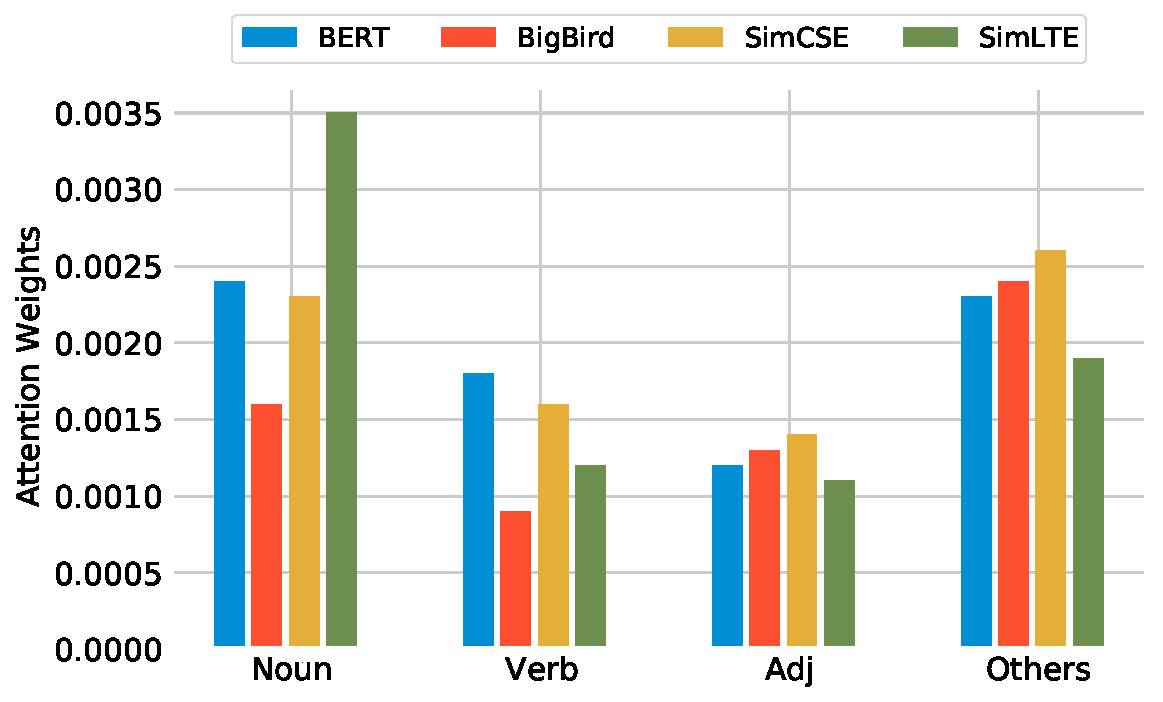
\includegraphics[width=0.8\linewidth]{fig/attentions.pdf}
% \caption{Attention weights from different models on the NYT dataset.}  
% \label{attentions}
% \end{figure}

% We compute the attention weights for Transformers as follows:
% (1) we first extract the attention weights between \texttt{[CLS]} token and all the other tokens;
% (2) we compute the averaged weights along different heads in multi-head attention;
% (3) the attention weights of the last layer in Transformers are used as the weights for words.
% Averaged values are computed for nouns, verbs, adjectives, and other words.

\end{document}
